\subsection{Pipeline}
\label{sec:methods_pipeline}

This research project follows a pipeline and general strategies proposed in
Lopez de Prado book (\cite{lopez_de_prado}) which do not differ significantly
from any other machine learning pipeline although there are a few key points
worth to mention and explain because they are not intuitively derived by
inspection. As commented before, there are two models:

\begin{itemize}
  \item Primary model: it outputs the buy and sell signals based on a certain
        set of features. We will further discuss this model in section \ref{sec:methods_pipeline_primary_model},
        however it involves a momentum based strategy computed out of the
        crossing events of two different speeds moving average signals (as
        initially introduced in \ref{sec:intro_fundamental_trading_strategies}).
  \item Secondary model: the first model outputs buy and sell signals based on
        prices, volumes, and other series. This second model is a machine
        learning model that will define the size of the position. The machine
        learning model will be explained in detailed section \ref{sec:methods_pipeline_secondary_model}.
  \item Training: training a machine learning model that uses time series as
        features requires special care to avoid leakage. Section \ref{sec:methods_pipeline_training}
        describes the involved methods to reduce the impact of leakage while
        preserving the performance of the model.
  \item Feature importance: it is expected that as part of the research process,
        more features than there are really required to develop the secondary
        model are used in the training stage. Once model's performance is satisfactory, features
        could be removed to obtain the right trade off between model complexity
        and required data. See section \ref{sec:methods_pipeline_feature_importance}
        for further details.
  \item Bet sizing: the secondary model outputs the confidence on the bet that 
        the primary model provided. This stage helps the financial analyst
        execute trades with consolidated sizes and avoids prompt operations that
        are not worth because transaction rates significantly damage the
        operation. See section \ref{sec:methods_pipeline_bet_sizing} for further
        details.
  \item Back testing: in this stage the strategy is stressed under different
        circumstances to evaluate its performance metrics. It is not a research
        tool to guide the training of the aforementioned models. Instead, it
        should be used as a benchmark tool and help the researcher to
        quantitatively compare different strategies. See section \ref{sec:methods_pipeline_backtesting}
        for further details.
\end{itemize}


In figure \ref{fig:pipeline} the previous stages are displayed in favor of
increased clarity. The training and feature selection stages are considered
inside the Secondary model process.

\begin{figure}[H]
    \centering
    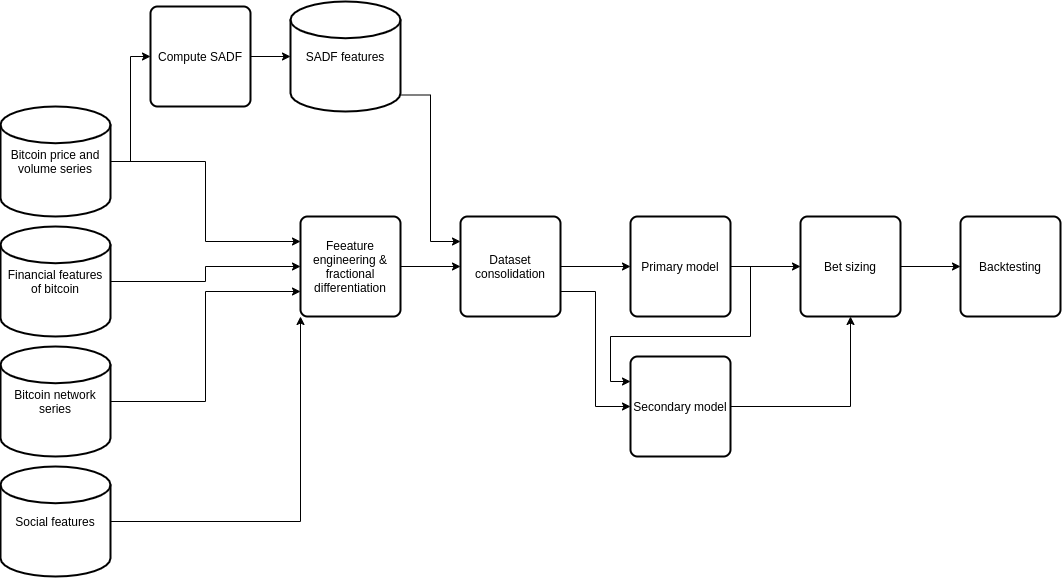
\includegraphics[width=\textwidth]{methods/images/pipeline.png}
    \caption{Financial machine learning pipeline used in this research project.}
    \label{fig:pipeline}
\end{figure}